% Options for packages loaded elsewhere
\PassOptionsToPackage{unicode}{hyperref}
\PassOptionsToPackage{hyphens}{url}
%
\documentclass[
]{article}
\usepackage{amsmath,amssymb}
\usepackage{iftex}
\ifPDFTeX
  \usepackage[T1]{fontenc}
  \usepackage[utf8]{inputenc}
  \usepackage{textcomp} % provide euro and other symbols
\else % if luatex or xetex
  \usepackage{unicode-math} % this also loads fontspec
  \defaultfontfeatures{Scale=MatchLowercase}
  \defaultfontfeatures[\rmfamily]{Ligatures=TeX,Scale=1}
\fi
\usepackage{lmodern}
\ifPDFTeX\else
  % xetex/luatex font selection
\fi
% Use upquote if available, for straight quotes in verbatim environments
\IfFileExists{upquote.sty}{\usepackage{upquote}}{}
\IfFileExists{microtype.sty}{% use microtype if available
  \usepackage[]{microtype}
  \UseMicrotypeSet[protrusion]{basicmath} % disable protrusion for tt fonts
}{}
\makeatletter
\@ifundefined{KOMAClassName}{% if non-KOMA class
  \IfFileExists{parskip.sty}{%
    \usepackage{parskip}
  }{% else
    \setlength{\parindent}{0pt}
    \setlength{\parskip}{6pt plus 2pt minus 1pt}}
}{% if KOMA class
  \KOMAoptions{parskip=half}}
\makeatother
\usepackage{xcolor}
\usepackage[margin=1in]{geometry}
\usepackage{graphicx}
\makeatletter
\def\maxwidth{\ifdim\Gin@nat@width>\linewidth\linewidth\else\Gin@nat@width\fi}
\def\maxheight{\ifdim\Gin@nat@height>\textheight\textheight\else\Gin@nat@height\fi}
\makeatother
% Scale images if necessary, so that they will not overflow the page
% margins by default, and it is still possible to overwrite the defaults
% using explicit options in \includegraphics[width, height, ...]{}
\setkeys{Gin}{width=\maxwidth,height=\maxheight,keepaspectratio}
% Set default figure placement to htbp
\makeatletter
\def\fps@figure{htbp}
\makeatother
\setlength{\emergencystretch}{3em} % prevent overfull lines
\providecommand{\tightlist}{%
  \setlength{\itemsep}{0pt}\setlength{\parskip}{0pt}}
\setcounter{secnumdepth}{-\maxdimen} % remove section numbering
% definitions for citeproc citations
\NewDocumentCommand\citeproctext{}{}
\NewDocumentCommand\citeproc{mm}{%
  \begingroup\def\citeproctext{#2}\cite{#1}\endgroup}
\makeatletter
 % allow citations to break across lines
 \let\@cite@ofmt\@firstofone
 % avoid brackets around text for \cite:
 \def\@biblabel#1{}
 \def\@cite#1#2{{#1\if@tempswa , #2\fi}}
\makeatother
\newlength{\cslhangindent}
\setlength{\cslhangindent}{1.5em}
\newlength{\csllabelwidth}
\setlength{\csllabelwidth}{3em}
\newenvironment{CSLReferences}[2] % #1 hanging-indent, #2 entry-spacing
 {\begin{list}{}{%
  \setlength{\itemindent}{0pt}
  \setlength{\leftmargin}{0pt}
  \setlength{\parsep}{0pt}
  % turn on hanging indent if param 1 is 1
  \ifodd #1
   \setlength{\leftmargin}{\cslhangindent}
   \setlength{\itemindent}{-1\cslhangindent}
  \fi
  % set entry spacing
  \setlength{\itemsep}{#2\baselineskip}}}
 {\end{list}}
\usepackage{calc}
\newcommand{\CSLBlock}[1]{\hfill\break\parbox[t]{\linewidth}{\strut\ignorespaces#1\strut}}
\newcommand{\CSLLeftMargin}[1]{\parbox[t]{\csllabelwidth}{\strut#1\strut}}
\newcommand{\CSLRightInline}[1]{\parbox[t]{\linewidth - \csllabelwidth}{\strut#1\strut}}
\newcommand{\CSLIndent}[1]{\hspace{\cslhangindent}#1}
\ifLuaTeX
  \usepackage{selnolig}  % disable illegal ligatures
\fi
\usepackage{bookmark}
\IfFileExists{xurl.sty}{\usepackage{xurl}}{} % add URL line breaks if available
\urlstyle{same}
\hypersetup{
  pdftitle={SCC.461 Report},
  pdfauthor={-----},
  hidelinks,
  pdfcreator={LaTeX via pandoc}}

\title{SCC.461 Report}
\author{36827814}
\date{2025-01-19}

\begin{document}
\maketitle

\begin{verbatim}
## -- Attaching core tidyverse packages ------------------------ tidyverse 2.0.0 --
## v dplyr     1.1.4     v readr     2.1.5
## v forcats   1.0.0     v stringr   1.5.1
## v ggplot2   3.5.1     v tibble    3.2.1
## v lubridate 1.9.4     v tidyr     1.3.1
## v purrr     1.0.2     
## -- Conflicts ------------------------------------------ tidyverse_conflicts() --
## x dplyr::filter() masks stats::filter()
## x dplyr::lag()    masks stats::lag()
## i Use the conflicted package (<http://conflicted.r-lib.org/>) to force all conflicts to become errors
## here() starts at D:/SCC.461 FINAL PROJECT
## 
## 
## Attaching package: 'gridExtra'
## 
## 
## The following object is masked from 'package:dplyr':
## 
##     combine
\end{verbatim}

\subsection{Abstract}\label{abstract}

This report examines the finds of the usage of two Decision Tree
Classifiers on three sets of data. It will provide analysis in two
areas. The first area focuses on the computational aspects that went
into training these Decision Tree Classifiers and the second area,
analyses the machine learning aspects themselves before forming some
conclusions about the classifier and data from these two separate areas.

\subsection{Introduction}\label{introduction}

This report examines data generated by two Decision Tree Classifiers.
The first Decision Tree Classifier was created and implemented by us and
the second Decision Tree Classifier was implemented from the
SKLearn.tree library. The results of which are compared later during the
Results section. The first decision tree (referred to as DT-One) was
created on the system specifications listed below:

\begin{verbatim}
System: Windows
Release: 10
Version: 10.0.19045
Machine: AMD64
Processor: Intel64 Family 6 Model 94 Stepping 3, GenuineIntel

CPU Information:
Processor: Intel64 Family 6 Model 94 Stepping 3, GenuineIntel
Physical Cores: 4
Logical Cores: 4

Memory Information:
Total Memory: 8467763200 bytes
Available Memory: 1055424512 bytes
Used Memory: 7412432896 bytes
Memory Utilization: 87.5%
\end{verbatim}

The second decision tree (DT-Two) was also ran on the same system. Both
of the DTs were also ran on another system, the specifications are
listed below:

\begin{verbatim}
System: Darwin
Release: 23.6.0
Version: Darwin Kernel Version 23.6.0: Fri Nov 15 15:13:28 PST 2024;
root:xnu-10063.141.1.702.7~1/RELEASE_X86_64
Machine: x86_64

CPU Information:
Processor: i386
Physical Cores: 6
Logical Cores: 12

Memory Information:
Total Memory: 17179869184 bytes
Available Memory: 6919766016 bytes
Used Memory: 8981368832 bytes
Memory Utilization: 59.7%
\end{verbatim}

\subsection{Methodology}\label{methodology}

DT-One is a custom Decision Tree classifier based off of the
Classification and Regression Tree (CART) algorithm. At the core of the
CART algorithm is a binary tree in with several different nodes. These
nodes have differing functions.

\begin{figure}
\centering
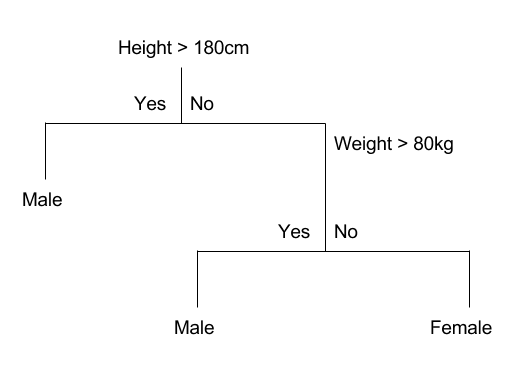
\includegraphics{Example-Decision-Tree.png}
\caption{Example Decision Tree from Brownlee {[}1{]}}
\end{figure}

\subsection{Results}\label{results}

\begin{figure}
\centering
\includegraphics{Report_files/figure-latex/unnamed-chunk-3-1.pdf}
\caption{Boxplot of Iris Data using DT-One and DT-Two}
\end{figure}

\subsection{Discussion}\label{discussion}

\subsection{Conclusion}\label{conclusion}

\subsection{Acknowledgements}\label{acknowledgements}

\subsection*{Bibliography}\label{bibliography}
\addcontentsline{toc}{subsection}{Bibliography}

\phantomsection\label{refs}
\begin{CSLReferences}{0}{0}
\bibitem[\citeproctext]{ref-exampledt}
\CSLLeftMargin{{[}1{]} }%
\CSLRightInline{J. Brownlee, {``Classification and regression trees for
machine learning.''} Machine Learning Mastery, Sep. 2017. Available:
\url{https://machinelearningmastery.com/classification-and-regression-trees-for-machine-learning/}}

\end{CSLReferences}

\end{document}
